% choose between screen or print "media" option in order to render more or less colored pages
\documentclass[media=screen, open=right, fontsize=12pt, twoside]{SPhdThesis}
% open=right  => chapters always start on the right side of a double page, alternative: any
% twoside means the printing style. Affects position of the page number. Alternative: oneside
% draft => option to speed up rendering during edit, renders boxes instead of images
	\usepackage{natbib}

% PDF and title properties.
\SgSetTitle{Title}
\SgSetSubTitle{Subtitle}
\SgSetAuthor{Full Name}
\SgSetAuthorMatNr{xxxx}
\SgSetAuthorEmail{fse@kernschall.de}
\SgSetAuthorDegrees{current degree}
\SgSetYear{01.	November 2018}
\SgSetDegree{Degree aimed at}
%\SgSetDepartment{Sound for Picture}
%\SgSetUniversity{Film University Babelsberg Konrad Wolf}
\SgSetDeclarationDate{01. November 2018}
\SgSetUniversityLogo{./pictures/Logo_HFF_ohne_Adresse_besserer_Text_transparent.png}
\SgSetKeywords{Sound effects retrieval, Interface design, audio post-production, Web-development}
\SgSetSupervisors{Prof. Dr. One}{Prof. Dr. Two}
		
% The document.
\begin{document}
		\SgAddTitle %
		\clearpage{\pagestyle{empty}\cleardoublepage}
	\begin{frontmatter}
		\begin{acknowledgments}

Thanks everyone

\vspace{1.5cm}
Thank you.
\begin{flushright}

Sincerely yours,\\
\vspace{2cm}
	\SgIntAuthor
\end{flushright} 
\end{acknowledgments} %
		\SgIntClearDoublePage
		\center
\emph{What you can not find in the world, shall be your contribution.}
 
- Inspired by Herrmann Hesse %
		\begin{abstract}

This example thesis is meant to introduce you to a few basic commands that you will need to work with latex. Always look at the source code whenever there is some example, because the interesting stuff happens underneath the surface :)

I want to give you a head-start into writing your thesis with latex, because after some initial hurdles you need to take, it can make the formal stuff so much easier, scientifically more sophisticated an your document will be better readable and even smaller in size.

You find examples of pretty much all functionality that I needed when writing my masters thesis. This template is not written by me, but I added some modifications. Make sure to have a look at the .cls file, because this one is well commented and shows you how to quickly manipulate the look of your whole document with just a few arguments and commands.

Enjoy writing!

\end{abstract}
 %
		\SgAddToc %  Table of contents.
		\SgAddAbbrv % List of abbreviations
		\SgAddLof %  List of figures.
		\SgAddLot %  List of tables.
		\SgAddLos %  List of source codes (take a look at the "minted" package - requires python
%		\SgAddLoa %  List of algorithms.
	\end{frontmatter}
	\clearpage{\pagestyle{empty}\cleardoublepage}	
	
	\chapter{chapter 1}
\label{ch:chapter1}

I used the commercial Latex editor Texpad (1.8.9), because I needed to speed up the initial setup time.  To focus on the content and structure I first wrote a short draft with Markup. I was quite in a hurry when I found out, that Markup to Latex conversion is not that gapless as I hoped.

When everything went well you should see the following content:

\begin{itemize}
	\item Title page
	\item \textit{Blank Page}
	\item Acknowledgements
	\item \textit{Blank Page}
	\item Abstract
	\item \textit{Blank Page}
	\item Table of contents
	\item \textit{Blank Page}
	\item List of Abbreviations (nomenclature)
	\item \textit{Blank Page}
	\item List of Figures
	\item \textit{Blank Page}
	\item List of Tables
	\item \textit{Blank Page}
	\item List of source codes (listings)
	\item \textit{Blank Page}
	\item Chapter1
	\item Chapter2
	\item \textit{Blank Page}
	\item Chapter3
	\item References (Bibliography)
	\item Declaration
\end{itemize}

Internal links to other pages of the document should be green, external links (URLs) should appear blue. If you set the option media=print, these colors will be changed to black. You find this line in \textit{thesis.tex}.

To have source code linted (colored depending on input e.g. variables other than functions), have a look at the "minted" package on CTAN \href{http://tug.ctan.org/tex-archive/macros/latex/contrib/minted/minted.pdf}{here}.

\begin{verbatim}
\documentclass[media=screen]{SPhdThesis}
\end{verbatim}

You can speed up rendering by using only placeholders instead of images by adding the "draft" option:

\begin{verbatim}
\documentclass[media=screen, draft]{SPhdThesis}
\end{verbatim}



If you decide to get rid of an unnecessary part of the frontmatter, just comment it out in the main \.tex file: \(thesis.tex\). 

\begin{listing}
\begin{verbatim}
	\begin{frontmatter}
		\begin{acknowledgments}

Thanks everyone

\vspace{1.5cm}
Thank you.
\begin{flushright}

Sincerely yours,\\
\vspace{2cm}
	\SgIntAuthor
\end{flushright} 
\end{acknowledgments} %
		\SgIntClearDoublePage
		\center
\emph{What you can not find in the world, shall be your contribution.}
 
- Inspired by Herrmann Hesse %
		\begin{abstract}

This example thesis is meant to introduce you to a few basic commands that you will need to work with latex. Always look at the source code whenever there is some example, because the interesting stuff happens underneath the surface :)

I want to give you a head-start into writing your thesis with latex, because after some initial hurdles you need to take, it can make the formal stuff so much easier, scientifically more sophisticated an your document will be better readable and even smaller in size.

You find examples of pretty much all functionality that I needed when writing my masters thesis. This template is not written by me, but I added some modifications. Make sure to have a look at the .cls file, because this one is well commented and shows you how to quickly manipulate the look of your whole document with just a few arguments and commands.

Enjoy writing!

\end{abstract}
 %
		\SgAddToc %  Table of contents.
		\SgAddAbbrv % List of abbreviations
		\SgAddLof %  List of figures.
		\SgAddLot %  List of tables.
		\SgAddLos %  List of source codes
		\SgAddLoa %  List of algorithms.
	\end{frontmatter}
\end{verbatim}
\caption{Latex code in the main document \textit{thesis.tex}}
\label{lst:latexexample}
\end{listing}

\section{citation examples}
\label{sec:citeationexamples}

The exact styling used by the citation commands derives from the chosen .bst (bibtex style document).

Always think of proper citation - this is Author year style as defined in the .bst

\begin{verbatim}
	\cite{cooper_about_2014}
\end{verbatim}
Example:	
	\cite{cooper_about_2014}

But you can also only cite the year of a publication 

\begin{verbatim}
	\citeyear{cooper_about_2014}
\end{verbatim} 

Example:
	\citeyear{cooper_about_2014}

There is even a command to put the year in parenthesis 


\begin{verbatim}
	\citeyearpar{cooper_about_2014}.
\end{verbatim} 

Example:
\citeyearpar{cooper_about_2014}

To include a reference in the bibliography without having to cite it in the text, use:

\begin{verbatim}
	\nocite{cooper_about_2014}
\end{verbatim}

	or to include all entries inside the .bib file, even the not cited ones:

\begin{verbatim}
	\nocite*	
\end{verbatim}
\nocite*

% nomenclature example, for List of Abbreviations

Don't forget to feed your nomenclature:
Communication is the key to superior results, think of
computer interface (HCI\nomenclature{HCI}{Human Computer Interface}) aspects.


\section{Motivation}
\label{sec:ch01_motivation}

Always think of people you enjoy.
% 

\begin{wrapfigure}{r}{0.5\textwidth}
\begin{flushright}
\begin{minipage}[t]{0.47\textwidth}
\begin{flushright}
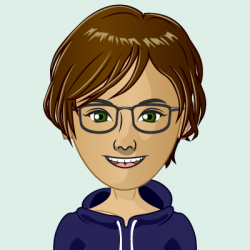
\includegraphics[width=\linewidth]{./pictures/Barb01.png}
\caption[Persona: Barbara]{Barbara:\newline Sound Desiger, Composer, Musician}
\label{fig:ch02_barbara}
\end{flushright}
\end{minipage}
\end{flushright}
\vspace{-12pt}
\end{wrapfigure}


\pagebreak

\section{Structure}
\label{subsec:ch01_structure}

In chapter \ref{ch:chapter2} you find a link back to this chapter.


	\chapter{Chapter 2}
\label{ch:chapter2}

Here ist the link back to chapter \ref{subsec:ch01_structure}.

\section{Section 1}
\label{sec:ch02_section01}

%\parbox[l]{width=0.5\textwidth}{
\begin{wrapfigure}{R}{0.5\textwidth}
\begin{minipage}[l][][l]{0.45\textwidth}
\vspace{-10pt}
\begin{itemize}
  \item Dialog 
  \begin{itemize}
	  \item Production-Sound 
	  \item Add. Dialog Recordings
	  \item Production Effects 
  \end{itemize}
  \item Foley
  \begin{itemize}
	  \item Movement
	  \item Steps
	  \item Props
	  \item Foley Effects
  \end{itemize}
  \item Hard Effects 
  \item Special Effects 
  \item Ambience 
  \begin{itemize}
  	\item Background
  	\item Foreground
  	\item Ambience Effects
  \end{itemize}
  \item Music
  \begin{itemize}
    \item Source Music
    \item Score Music
    \item Music Effects
  \end{itemize}
\end{itemize}%
\vspace{5pt}
\end{minipage}
\captionsetup{width=0.85\linewidth}
\caption[Layers of Film Sound]{Complex film-soundtracks usually apply variations of this layer structure
}
\vspace{-30pt}
\end{wrapfigure}

\paragraph{Special Effects} as a layer contains again multiple layers of
audio clips for each sound effect. A short car crash will be a composition of
screeching wheels, a sharp metal hit sound, a hit on a resonant large
wood box or steel barrel for increasing the physicality and impact and
some shattered glass across the street. Each of these can again be a
mixture of several sounds to create a feeling of the intended sonic
expression to the accompanying picture. This is the most demanding
layer in terms of using pre-recorded sound material. \textit{Sound Effects} are a vertisile category ranging from purely atmospheric and subconsciously effective undefined sound objects like drones to very present and narrative key sounds.
%\pagebreak
\paragraph{Ambience} or \emph{Atmo} is usually a mixture of longer noisy
field-recordings for building an appropriate background for the action
on screen. Also many single cues ("sweeteners") with more
distinguishable sounds are added to enhance the immersion of the film
for example bird calls, wood creaking, distant dog barking, traffic and
so on. This is the second layer where a large collection of sound effect
recordings are necessary to build a good soundtrack. 
\vspace{-11pt}

\paragraph{Foley} can be enhanced or complemented as well by pre-recorded material, perhaps of elements that were difficult to produce in a studio (for example \textit{Hard Effects} like door sounds). Or maybe the low budget does not allow a human foley artist to be payed for his or
her performance, so the editor is in charge of delivering movement and prop
sounds for the scene.

\paragraph{Dialog} needs from time to time a very specific background noise
to stitch gaps between the edges of the edited audio regions that could
be found in a library.

\paragraph{Music} composers frequently use sound effects as well, since the
boundary between sound design and music is fluid, but we will not
concentrate on this exiting topic here. We assume here that composers
and sound designers have the same way of accessing sound effects
collections.

\paragraph{Games and Animations} also have a high demand for sound effects, maybe even
higher, as there is no production sound at all - everything is silent at the
beginning and has to be generated and assigned. In game audio the
mentioned layers are also used, but as the mix is dynamically generated
depending on in-game parameters, this separation often becomes less
obvious in editing projects.

Barbara could certainly write a book of her own. So we will concentrate on the relevant aspects of searching for sounds in her
storage devices.

\pagebreak

\subsection{Subsection 1.1}
\label{subsec:subsection}


\begin{table}[h]
%\caption{Feature frequency among various search related software solutions}
\label{tab:ch04_app_freq}
	\centering
	\begin{tabularx}{\linewidth}{p{0.22\linewidth}||p{0.13\linewidth}|p{0.08\linewidth}|p{0.11\linewidth}|p{0.08\linewidth}|p{0.08\linewidth}|p{0.11\linewidth}}
%		\toprule
		& Spreadsheet view & Grid view & Color mapping & Scatter-plot & Glyphs & Inline Preview\tabularnewline
		\toprule
%		\endhead
		Metadata Management Software & 8 & 1 & 1 & 0 & 0 & 2\tabularnewline
		Interactive Visualization Software & 3 & 5 & 6 & 6 & 3 & 5\tabularnewline
	\bottomrule
	\end{tabularx}
	\caption[Metadata application feature frequency]{Metadata application feature frequency\footnotemark}
	\label{tab:appfeatfreq}
\end{table}
\footnotetext{ you can even have footnotes in captions! See: \ref{fig:ch02_barbara} and \ref{fig:tristimequations} on page \pageref{fig:tristimequations}}


%\pagebreak



	\SgIntClearDoublePage % sometimes it is neccessary to insert a clear page in order to open the chapter right...
	\chapter{Applied Methods in Sound Search Interfaces}
\label{ch:relatedworks}


Use the optional positional agrument to place the figure on top [t], bottom [b] or just somewhere here [h] or exactly here [H] or [h!].

The \begin{verbatim}
	$$
\end{verbatim} sign opens and closes a miniature math environment where you can easily write formulas in a scientific way. Have a look at the source code for the example in figure \ref{fig:tristimequations}.


\begin{figure}[h]
$$
T1=\frac{a_1}{\sum_{h} a_h} = Red
$$
$$
T2 = \frac{a_2+a_3+a_4}{\sum_{h} a_h} = Green
$$
$$
T3=\frac{\sum_{h=5}^H a_h}{\sum_{h} a_h} = Blue
$$
$a_h$ = harmonic with index h

$H$ = highest harmonic of the spectrum
\caption{Tristiumulus equations}
\label{fig:tristimequations}
\end{figure}




\begin{listing}

\begin{verbatim}
// comments are colored differently than the actual code

import Sun from 'galaxy';
const speedOfLight = 9999999999999
Sun.shine(speedOfLight)

export Sun
\end{verbatim} 
\caption{Javascript example}
\label{lst:jsexample}
\end{listing}



	\bibliographystyle{dinat_en}
	\bibliography{bibliography}
%	\SgIncludeBib{bibliography}

	\SgAddDeclaration %

\end{document}
